\chapter{Analisi dei requisiti}
\label{cap:analisi-requisiti}

\intro{In questo capitolo viene esposta l'analisi dei requisiti effettuata durante lo stage, dove si
 vanno ad illustrare le funzionalità tramite casi d'uso e requisiti identificati, con l'obiettivo di creare un'immagine
 più chiara e definita del sistema.
 }\\

\section{Descrizione dell'applicazione}

\section{Casi d'uso}

La seguente sezione illustra i casi d'uso individuati durante l'analisi dei requisiti. 
% \begin{figure}[!h] 
%     \centering 
%     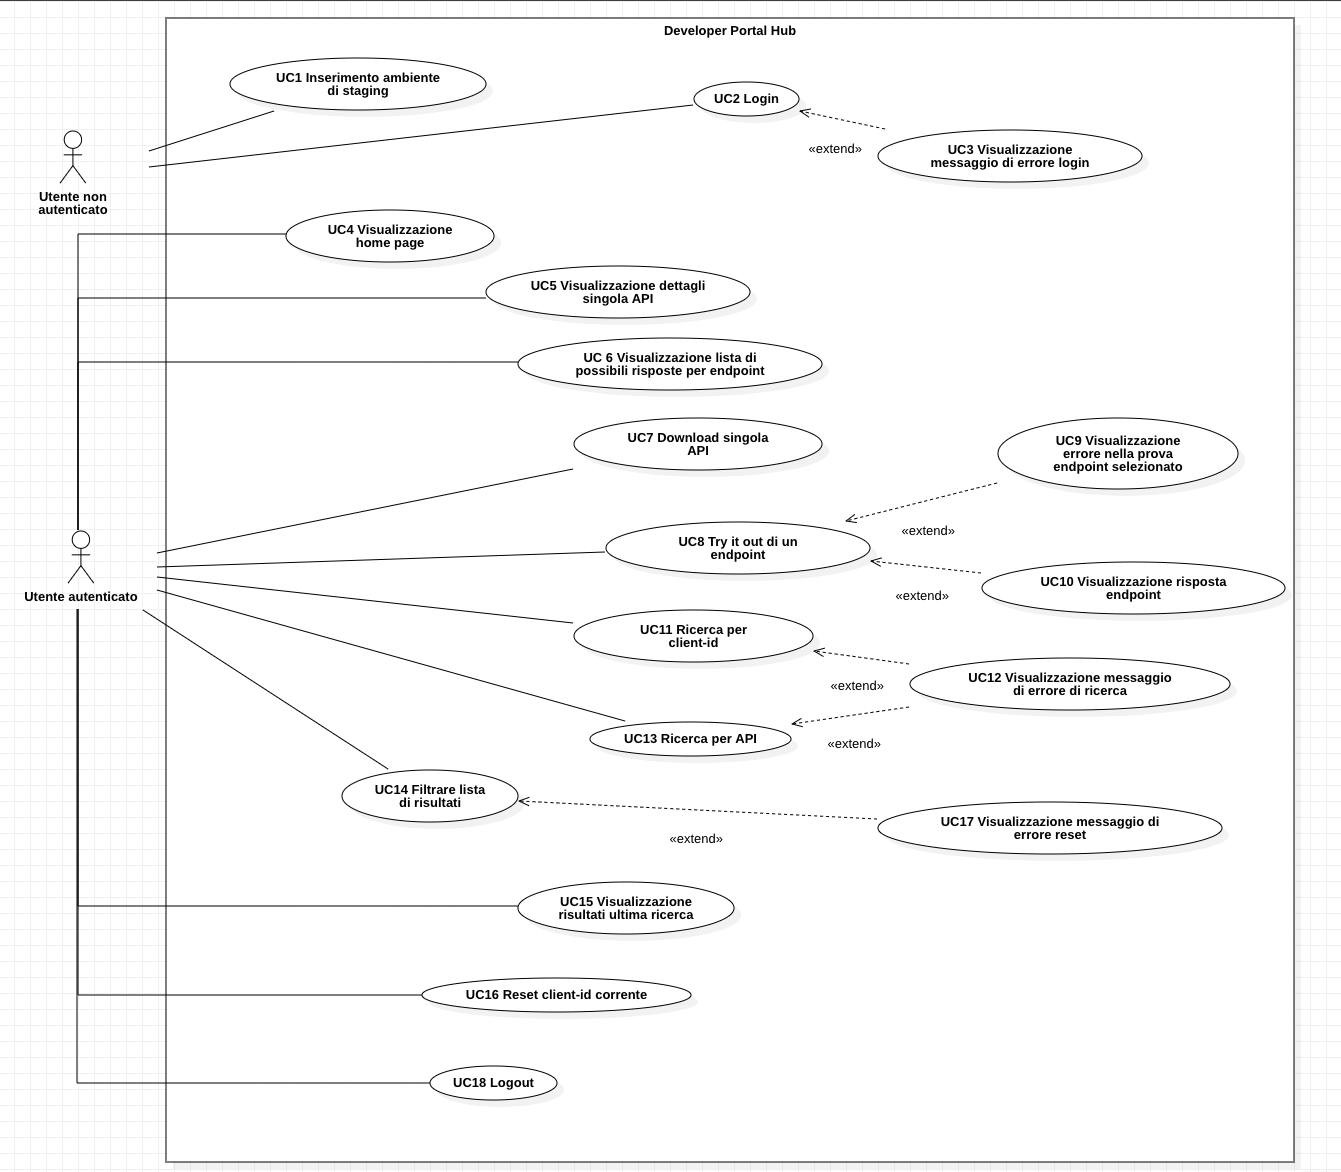
\includegraphics[width=0.9\columnwidth]{usecase/scenario-principale} 
%     \caption{Use Case - UC0: Scenario principale}
% \end{figure}

\subsection{Notazione utilizzata}

\subsection{Attori}


\subsection{Descrizione del sistema}

% UC 1 - Inserimento ambiente di staging
\begin{usecase}{}{}\label{uc:}
    \usecaseactors{Utente autenticato}
    \usecasepre{}
    \usecasedesc{}
    \usecasepost{}

    \usecasemain{}
        \begin{enumerate}
            \item 
        \end{enumerate}

\end{usecase}

% UC 2 - Login
\begin{usecase}{2}{Login}\label{uc:login}
    \usecaseactors{Utente non autenticato}
    \usecasepre{ L'utente possiede un account valido per autenticazione tramite microsoft 365 che appartiene al gruppo autorizzato per il login al portale. Inoltre l'utente non è autenticato e si trova nella pagina di login}
    \usecasedesc{L'utente vuole accedere al portale e deve inserire le proprie credenziali per accedervi}
    \usecasepost{L'utente è autenticato correttamente e può procedere con l'utilizzo di tutte le funzionalità disponibili all'interno del portale}

    \usecasemain{}
        \begin{enumerate}
            \item L'utente inserisce la propria e-mail;
            \item L'utente inserisce la propria password.
        \end{enumerate}

    \usecaseext{}
    \begin{enumerate}
        \item Visualizzazione messaggio di errore login UC3.
    \end{enumerate}

    \usecasegen{}
    \begin{enumerate}
        \item Inserimento e-mail UC2.1;
        \item Inserimento password UC2.2.
    \end{enumerate}

\end{usecase}


% UC 2.1 - Inserimento e-mail
\begin{usecase}{2.1}{Inserimento e-mail}\label{uc:inserimento-email}
    \usecaseactors{Utente non autenticato}
    \usecasepre{L'utente possiede un account valido per autenticazione tramite microsoft 365 che appartiene al gruppo autorizzato per il login al portale. Inoltre l'utente non è autenticato e si trova nella pagina di login}
    \usecasedesc{L'utente deve inserire la propria e-mail per autenticarsi al portale}
    \usecasepost{L'utente ha inserito la propria e-mail, può quindi procedere a completare il processo di autenticazione}

    \usecasemain{}
        \begin{enumerate}
            \item L'utente inserisce nell'apposito campo la propria e-mail.
        \end{enumerate}

\end{usecase}


% UC 2.2 - Inserimento password
\begin{usecase}{2.2}{Inserimento password}\label{uc:inserimento-password}
    \usecaseactors{Utente non autenticato}
    \usecasepre{L'utente possiede un account valido per autenticazione tramite microsoft 365 che appartiene al gruppo autorizzato per il login al portale. Inoltre l'utente non è autenticato e si trova nella pagina di login}
    \usecasedesc{Descrizione → L'utente deve inserire la propria password per autenticarsi al portale}
    \usecasepost{L'utente ha inserito la propria password e può concludere il processo di autenticazione}

    \usecasemain{}
        \begin{enumerate}
            \item L'utente inserisce nell'apposito campo la propria password.
        \end{enumerate}

\end{usecase}


% UC 3 - Visualizzazione messggio di errore login
\begin{usecase}{3}{Visualizzazione messggio di errore login}\label{uc:visualizzazione-errore-login}
    \usecaseactors{Utente non autenticato}
    \usecasepre{L'utente ha inserito una tra le due credenziali email o password in modo errato}
    \usecasedesc{L'utente ha inserito una tra le due credenziali errate}
    \usecasepost{L'utente ha inserito una tra le due credenziali errate}

    \usecasemain{}
        \begin{enumerate}
            \item L'utente visualizza un messaggio di errore che lo informa che una delle credenziali che ha inserito per autenticarsi al portale è sbagliata.
        \end{enumerate}

\end{usecase}

% UC 4 - Visualizzazione home page
\begin{usecase}{4}{Visualizzazione home page}\label{uc:visualizzasioen-home-page}
    \usecaseactors{Utente autenticato}
    \usecasepre{L'utente è autenticato ed è stato reindirizzato alla pagina principale del portale}
    \usecasedesc{L'utente visualizza la pagina principale del portale}
    \usecasepost{L'utente ha visualizzato la pagina principale del portale}

    \usecasemain{}
        \begin{enumerate}
            \item L'utente visualizza la pagina principale del portale.
        \end{enumerate}

    \usecasegen{}
        \begin{enumerate}
            \item Visualizzazione lista APIs disponibili UC4.1;
            \item Visualizzazione client-id di default per l'ambiente scelto UC4.2.
            \item Visualizzazione dettagli utente autenticato UC4.3. % ?????????????????????????
        \end{enumerate}

\end{usecase}

% UC 4.1 - Visualizzazione lista APIs disponibili
\begin{usecase}{4.1}{Visualizzazione lista APIs disponibili}\label{uc:visualizzazione-lista-apis-disponibili}
    \usecaseactors{Utente autenticato}
    \usecasepre{L'utente è autenticato ed è stato reindirizzato alla pagina principale del portale}
    \usecasedesc{L'utente visualizza la lista di API disponibili per la consultazione all'interno del portale}
    \usecasepost{L'utente ha visualizzato la lista di API disponibili nel portale}

    \usecasemain{}
        \begin{enumerate}
            \item L'utente visualizza la lista di API disponibili nel portale.
        \end{enumerate}

\end{usecase}

% UC 4.2 - Visualizzazione client-id di default per l'ambiente scelto
\begin{usecase}{4.2}{Visualizzazione client-id di default per l'ambiente scelto}\label{uc:visualizzazione-client-id-di-default-per-lambiente-scelto}
    \usecaseactors{Utente autenticato}
    \usecasepre{L'utente è autenticato ed è stato reindirizzato alla pagina principale del portale}
    \usecasedesc{L'utente visualizza il client id di default impostato nell'ambiente corrente}
    \usecasepost{L'utente ha visualizzato il client id di default impostato nell'ambiente corrente}

    \usecasemain{}
        \begin{enumerate}
            \item L'utente visualizza il client id di default impostato nell'ambiente corrente.
        \end{enumerate}

\end{usecase}


% % UC 4.3 Visualizzazione dettagli utente autenticato
\begin{usecase}{}{}\label{uc:}
    \usecaseactors{Utente autenticato}
    \usecasepre{}
    \usecasedesc{}
    \usecasepost{}

    \usecasemain{}
        \begin{enumerate}
            \item 
        \end{enumerate}

\end{usecase}

% UC 5 Visualizzazione dettaglio singola API
\begin{usecase}{5}{Visualizzazione dettaglio singola API}\label{uc:visualizzazione-dettaglio-singola-api}
    \usecaseactors{Utente autenticato}
    \usecasepre{L'utente è autenticato e si trova nella pagina principale del portale}
    \usecasedesc{L'utente vuole visualizzare la pagina di dettaglio di una singola API}
    \usecasepost{L'utente ha visualizzato la pagina di dettaglio di una singola API tra quelle presenti nel portale}

    \usecasemain{}
        \begin{enumerate}
            \item L'utente clicca su una delle API presenti nella lista di API disponibili;
            \item L'utente visualizza la pagina di dettaglio di una singola API tra quelle presenti nel portale.
        \end{enumerate}

    \usecasegen{}
        \begin{enumerate}
            \item Visualizzaazione lista endpoint disponibili UC5.1;
            \item Visualizzazione sezione models dell'endpoint UC5.2. %?????????????????????????????????????????????
        \end{enumerate}


\end{usecase}


% UC 5.1 Visualizzazione lista endpoint disponibili
\begin{usecase}{5.1}{Visualizzazione lista endpoint disponibili}\label{uc:visualizzazione-lista-endpoint-disponibili}
    \usecaseactors{Utente autenticato}
    \usecasepre{L'utente è autenticato e sta visualizzando la pagina di dettaglio di una singola API}
    \usecasedesc{L'utente vuole visualizzare la lista completa di endpoint disponibili per l'API}
    \usecasepost{L'utente visualizza la lista completa di endpoint disponibili per l'API}

    \usecasemain{}
        \begin{enumerate}
            \item L'utente visualizza la pagina di dettaglio di una singola API tra quelle presenti nel portale;
            \item L'utente visualizza la lista completa di endpoint disponibili per l'API che ha selezionato.
        \end{enumerate}


\end{usecase}

%
% Visualizzazione models???
% categorie di endpoints??
%

% UC 5.1.1 Visualizzazione dettaglio singolo endpoint
\begin{usecase}{5.1.1}{Visualizzazione dettaglio singolo endpoint}\label{uc:visualizzazione-dettaglio-singolo-endpoint}
    \usecaseactors{Utente autenticato}
    \usecasepre{L'utente è autenticato, sta visualizzando la pagina di dettaglio di una singola API contenente la lista di endpoint disponibili}
    \usecasedesc{L'utente vuole visualizzare la pagina di dettaglio di un singolo endpoint}
    \usecasepost{L'utente visualizza la pagina di dettaglio di un singolo endpoint}

    \usecasemain{}
        \begin{enumerate}
            \item L'utente clicca sullo specifico endpoint che vuole visualizzare;
            \item L'utente visualizza i dettagli disponibili per l'endpoint selezionato.
        \end{enumerate}


\end{usecase}


% UC 
\begin{usecase}{}{}\label{uc:}
    \usecaseactors{Utente autenticato}
    \usecasepre{}
    \usecasedesc{}
    \usecasepost{}

    \usecasemain{}
        \begin{enumerate}
            \item 
        \end{enumerate}


\end{usecase}


% UC 6 Download singola API
\begin{usecase}{6}{Download singola API}\label{uc:download-singola-api}
    \usecaseactors{Utente autenticato}
    \usecasepre{L'utente è autenticato ed ha selezionato una API dalla lista di API disponibili}
    \usecasedesc{L'utente vuole poter scaricare in formato yaml un API dal portale}
    \usecasepost{L'utente ha scaricato in formato yaml un API dal portale}

    \usecasemain{}
        \begin{enumerate}
            \item L'utente scarica il formato yaml di un API dal portale, tra quelle disponibili;
            \item Una nuova pagina si apre e il download dell'API viene eseguito;
            \item Il nome del file è già impostato con il nome dell'API scaricata.
        \end{enumerate}

\end{usecase}

% Visualizzazione descrizione del dettaglio endpoint / api

% UC 7 Try it out di un endpoint
\begin{usecase}{7}{Try it out di un endpoint}\label{uc:try-it-out-di-un-endpoint}
    \usecaseactors{Utente autenticato}
    \usecasepre{L'utente è autenticato, sta visualizzando i dettagli di un singolo endpoint di un API disponibile nel portale}
    \usecasedesc{L'utente vuole poter provare l'endpoint selezionato}
    \usecasepost{L'utente ha provato l'endpoint selezionato}

    \usecasemain{}
        \begin{enumerate}
            \item L'utente ha selezionato una determinata API
            \item L'utente ha selezionato un determinato endpoint di quell'API
            \item L'utente ha cliccato sul pulsante per provare l'endpoint selezionato
        \end{enumerate}

    \usecaseext{}
        \begin{enumerate}
            \item Visualizzazione errore nella prova dell'endpoint selezionato UC8;
            \item Visualizzazione risposta dell'endpoint selezionato UC9;
            \item Visualizzazione lista di possibili risposte per l'endpoint selezionato UC10.
        \end{enumerate}

    \usecasegen{}
        \begin{enumerate}
            \item Inserimento parametri per try it out endpoint UC7.1;
            \item Definire campi aggiuntivi per try it out endpoint UC7.2.
        \end{enumerate}

\end{usecase}


% UC 7.1 Inserimento parametri necessari per la prova dell'endpoint     
\begin{usecase}{7.1}{Inserimento parametri per try it out endpoint}\label{uc:inserimento-parametri-per-try-it-out-endpoint}
    \usecaseactors{Utente autenticato}
    \usecasepre{L'utente è autenticato, sta visualizzando la schermata di try it out nella sezione di inserimento dei parametri}
    \usecasedesc{L'utente vuole poter inserire i parametri necessari per la prova dell'endpoint}
    \usecasepost{L'utente ha inserito i parametri necessari alla chiamata verso l'endpoint}

    \usecasemain{}
        \begin{enumerate}
            \item L'utente è nella sezione di prova dell'endpoint che ha selezionato;
            \item L'utente inserisce i parametri richiesti per la chiamata verso l'endpoint selezionato.
        \end{enumerate}

\end{usecase}


% UC 7.2 Definire campi aggiuntivi per try it out endpoint
\begin{usecase}{}{}\label{uc:}
    \usecaseactors{Utente autenticato}
    \usecasepre{}
    \usecasedesc{}
    \usecasepost{}

    \usecasemain{}
        \begin{enumerate}
            \item 
        \end{enumerate}

\end{usecase}

% UC 8 Visualizzazione errore nella prova dell'endpoint selezionato
\begin{usecase}{8}{Visualizzazione errore nella prova dell'endpoint selezionato}\label{uc:visualizzazione-errore-nella-prova-dell-endpoint-selezionato}
    \usecaseactors{Utente autenticato}
    \usecasepre{}
    \usecasedesc{}
    \usecasepost{}

    \usecasemain{}
        \begin{enumerate}
            \item 
        \end{enumerate}

\end{usecase}


% UC 9 Visualizzazione risposta dell'endpoint selezionato
\begin{usecase}{}{}\label{uc:}
    \usecaseactors{Utente autenticato}
    \usecasepre{}
    \usecasedesc{}
    \usecasepost{}

    \usecasemain{}
        \begin{enumerate}
            \item 
        \end{enumerate}

\end{usecase}


% UC 10 Visualizzazione lista di possibili risposte per l'endpoint selezionato
\begin{usecase}{}{}\label{uc:}
    \usecaseactors{Utente autenticato}
    \usecasepre{}
    \usecasedesc{}
    \usecasepost{}

    \usecasemain{}
        \begin{enumerate}
            \item 
        \end{enumerate}

\end{usecase}


% UC 11 Ricerca per client-id
\begin{usecase}{}{}\label{uc:}
    \usecaseactors{Utente autenticato}
    \usecasepre{}
    \usecasedesc{}
    \usecasepost{}

    \usecasemain{}
        \begin{enumerate}
            \item 
        \end{enumerate}

    \usecaseext{}
        \begin{enumerate}
            \item Visualizzazione messaggio di errore di ricerca UC 12.
        \end{enumerate}

    \usecasegen{}
        \begin{enumerate}
            \item Inserimento client-id per ricerca UC11.1.
        \end{enumerate}

\end{usecase}


% % UC 11.1 Inserimento client-id per ricerca
\begin{usecase}{}{}\label{uc:}
    \usecaseactors{Utente autenticato}
    \usecasepre{}
    \usecasedesc{}
    \usecasepost{}

    \usecasemain{}
        \begin{enumerate}
            \item 
        \end{enumerate}

\end{usecase}


% % UC 12 Visualizzazione messaggio di errore di ricerca
\begin{usecase}{}{}\label{uc:}
    \usecaseactors{Utente autenticato}
    \usecasepre{}
    \usecasedesc{}
    \usecasepost{}

    \usecasemain{}
        \begin{enumerate}
            \item 
        \end{enumerate}

\end{usecase}


% UC 13 Ricerca per api
\begin{usecase}{}{}\label{uc:}
    \usecaseactors{Utente autenticato}
    \usecasepre{}
    \usecasedesc{}
    \usecasepost{}

    \usecasemain{}
        \begin{enumerate}
            \item 
        \end{enumerate}

    \usecaseext{}
        \begin{enumerate}
            \item Visualizzazione messaggio di errore di ricerca UC 12.
        \end{enumerate}

    \usecasegen{}
        \begin{enumerate}
            \item Inserimento nome api per ricerca UC13.1.
        \end{enumerate}

\end{usecase}



% UC 13.1 Inserimento nome api per ricerca
\begin{usecase}{}{}\label{uc:}
    \usecaseactors{Utente autenticato}
    \usecasepre{}
    \usecasedesc{}
    \usecasepost{}

    \usecasemain{}
        \begin{enumerate}
            \item 
        \end{enumerate}

\end{usecase}



% % UC 14 Filtrare lista di risultati per client-id
% \begin{usecase}{}{}\label{uc:}
%     \usecaseactors{Utente autenticato}
%     \usecasepre{}
%     \usecasedesc{}
%     \usecasepost{}

%     \usecasemain{}
%         \begin{enumerate}
%             \item 
%         \end{enumerate}

% \end{usecase}



% UC 15 Reset client-id corrente
\begin{usecase}{}{}\label{uc:}
    \usecaseactors{Utente autenticato}
    \usecasepre{}
    \usecasedesc{}
    \usecasepost{}

    \usecasemain{}
        \begin{enumerate}
            \item 
        \end{enumerate}

    \usecaseext{}
        \begin{enumerate}
            \item Visualizzazione messaggio di errore reset UC 16.
        \end{enumerate}

\end{usecase}


% UC 16 Logout
\begin{usecase}{}{}\label{uc:}
    \usecaseactors{Utente autenticato}
    \usecasepre{}
    \usecasedesc{}
    \usecasepost{}

    \usecasemain{}
        \begin{enumerate}
            \item 
        \end{enumerate}

\end{usecase}


% % UC 
% \begin{usecase}{}{}\label{uc:}
%     \usecaseactors{Utente autenticato}
%     \usecasepre{}
%     \usecasedesc{}
%     \usecasepost{}

%     \usecasemain{}
%         \begin{enumerate}
%             \item 
%         \end{enumerate}

% \end{usecase}




\section{Tracciamento dei requisiti}

Da un'attenta analisi dei requisiti e degli use case effettuata sul progetto è stata stilata la tabella che traccia i requisiti in rapporto agli use case.\\
% Sono stati individuati diversi tipi di requisiti e si è quindi fatto utilizzo di un codice identificativo per distinguerli.\\
% Il codice dei requisiti è così strutturato R(F/Q/V)(N/D/O) dove:
% \begin{enumerate}
% 	\item[R =] requisito
%     \item[F =] funzionale
%     \item[Q =] qualitativo
%     \item[V =] di vincolo
%     \item[N =] obbligatorio (necessario)
%     \item[D =] desiderabile
%     \item[Z =] opzionale
% \end{enumerate}
% Nelle tabelle \ref{tab:requisiti-funzionali}, \ref{tab:requisiti-qualitativi} e \ref{tab:requisiti-vincolo} sono riassunti i requisiti e il loro tracciamento con gli use case delineati in fase di analisi.

% \newpage

% \begin{table}%
% \caption{Tabella del tracciamento dei requisti funzionali}
% \label{tab:requisiti-funzionali}
% \begin{tabularx}{\textwidth}{lXl}
% \hline\hline
% \textbf{Requisito} & \textbf{Descrizione} & \textbf{Use Case}\\
% \hline
% RFN-1     & L'interfaccia permette di configurare il tipo di sonde del test & UC1 \\
% \hline
% \end{tabularx}
% \end{table}%

% \begin{table}%
% \caption{Tabella del tracciamento dei requisiti qualitativi}
% \label{tab:requisiti-qualitativi}
% \begin{tabularx}{\textwidth}{lXl}
% \hline\hline
% \textbf{Requisito} & \textbf{Descrizione} & \textbf{Use Case}\\
% \hline
% RQD-1    & Le prestazioni del simulatore hardware deve garantire la giusta esecuzione dei test e non la generazione di falsi negativi & - \\
% \hline
% \end{tabularx}
% \end{table}%

% \begin{table}%
% \caption{Tabella del tracciamento dei requisiti di vincolo}
% \label{tab:requisiti-vincolo}
% \begin{tabularx}{\textwidth}{lXl}
% \hline\hline
% \textbf{Requisito} & \textbf{Descrizione} & \textbf{Use Case}\\
% \hline
% RVO-1    & La libreria per l'esecuzione dei test automatici deve essere riutilizzabile & - \\
% \hline
% \end{tabularx}
% \end{table}%
